\begin{pastexam}[label={px:ntust-109-ice-04}]{臺科大資工所 109 學年度 第 4 題}
（問答）

There are 11 elements (or nodes) in a binary search tree (\textit{BST}). The integer keys of the
elements are 4, 28, 31, 7, 10, 25, 1, 16, 19, 13, 22 (the order is irrelevant). Assume that the left
subtree and the right subtree of the root in the \textit{BST} are both complete binary trees with 3
elements and 7 elements, respectively.
\begin{enumerate}[label=(\alph*)]
\item What is the key of the root in the \textit{BST}? (4\%)
\item Draw the entire \textit{BST}. (5\%)
\end{enumerate}
\end{pastexam}

\begin{pastsoln}
答案：(a) $10$；(b) 見下圖。

先把鍵值排好：$1, 4, 7, 10, 13, 16, 19, 22, 25, 28, 31$。 二元搜尋樹的中序走訪就是這個順序
（資結書定理~9.1），而中序是「左子樹、根、右子樹」，所以左子樹佔最前面幾個、根接在後面、
右子樹佔最後面幾個。

\textbf{(a)} 左子樹有 $3$ 個節點，就是最小的三個 $1, 4, 7$；根是第 $4$ 小的 $10$；右子樹是剩下的
$7$ 個 $13, 16, 19, 22, 25, 28, 31$。 這也是資結書第~9.4~節「子樹大小決定名次」的想法：根的名次
是左子樹大小加一，$3 + 1 = 4$。

\textbf{(b)} 再對兩棵子樹用同一個想法。 有 $3$ 個節點的完整二元樹形狀固定：根加兩個子節點，
所以根是中間的 $4$，左右是 $1$ 和 $7$。 有 $7$ 個節點的完整二元樹是高度 $3$ 的完美二元樹，
根的左右子樹各有 $3$ 個節點：根是第 $4$ 個 $22$，左子樹 $\{13, 16, 19\}$ 以 $16$ 為根，右子樹
$\{25, 28, 31\}$ 以 $28$ 為根。
\begin{center}
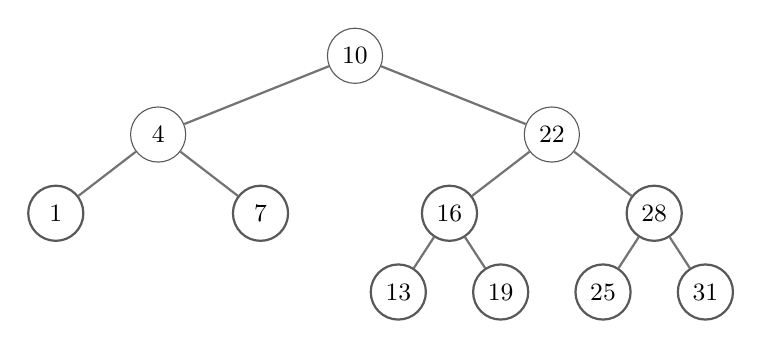
\begin{tikzpicture}[level distance=10mm,
  every node/.style={circle,draw=black!65,minimum size=7mm,inner sep=0pt,font=\small},
  edge from parent/.style={draw=black!55,thick},
  level 1/.style={sibling distance=50mm},
  level 2/.style={sibling distance=26mm},
  level 3/.style={sibling distance=13mm}]
\node {10}
  child {node {4}
    child {node {1}}
    child {node {7}}}
  child {node {22}
    child {node {16}
      child {node {13}}
      child {node {19}}}
    child {node {28}
      child {node {25}}
      child {node {31}}}};
\end{tikzpicture}
\end{center}
中序走訪這棵樹得到 $1, 4, 7, 10, 13, 16, 19, 22, 25, 28, 31$，由小到大，確實是二元搜尋樹；
左子樹 $3$ 個、右子樹 $7$ 個節點，兩棵都是完整二元樹。 因為每一層的根都由「左子樹有幾個」
決定，這棵樹是唯一的。
\end{pastsoln}
